 \documentclass[a4paper,12pt]{article}
\usepackage[top=2cm, bottom=2cm, left=2cm, right=2.5cm]{geometry}
\usepackage[utf8]{inputenc}
\usepackage[brazil]{babel}
\usepackage{amsmath, amsfonts, amssymb}
\usepackage{pifont} % Usado para especificar os simbolos em \begin{itemize} \item
\usepackage{hyperref} % Usado para adicionar hiperlinks com o comando p.ex: \href{http://www.latex-tutorial.com}{LaTeX-Tutorial}.
\usepackage{times} % Para usar a fonte Times New Roman no documento inteiro
\usepackage{graphicx} % Para incluir no documento figuras
\usepackage{float}
\usepackage{caption} % Pacote para Legenda em figuras e tabelas ( Para acescentar "Fonte" e notas nas figuras e tabelas )
\usepackage[shortlabels]{enumitem} % Usado para que possamos especificar explicitamente os itens que queremos num \begin{enumerate} ... \end{enumerate}


\begin{document}

\title{{\huge Capítulo 21 - Análise Combinatória - Métodos de Contagem} \\ 
  \, \linebreak \linebreak \linebreak Exercícios Respondidos, Básicos, Complementares e Questões de Vestibular
}
\date{}

\maketitle 

\begin{figure}[htb]
 \centering
 
\includegraphics[scale=0.4]{../../imagens/FOTO-PERFIL-DANIEL-CLAUDINO-2020.png}
\end{figure}

\begin{center}
  \begin{large}
    {\huge Autor: Daniel de Lima Claudino \linebreak \linebreak} 
  \end{large}
\end{center}

\begin{flushright}
  \begin{small}
    {\large \textbf{Referência Bibliográfica}\\PAIVA, Manoel Rodrigues. \textbf{Matemática}. Vol. 2. São Paulo: Moderna, 2004.} 
  \end{small}
\end{flushright}

\vfill

\begin{center}
  \begin{large}
    Dezembro/2022
  \end{large}
  
\end{center}

\thispagestyle{empty} % Não numera esta página

\newpage
\setcounter{page}{0}

\tableofcontents

\listoffigures

\listoftables

\thispagestyle{empty}% Não numera esta página

\newpage

\section{Mapa Mental - Análise Combinatória}

\setcounter{figure}{0}
\begin{figure}[htb]
\centering
\caption{Mapa Mental - Análise Combinatória}
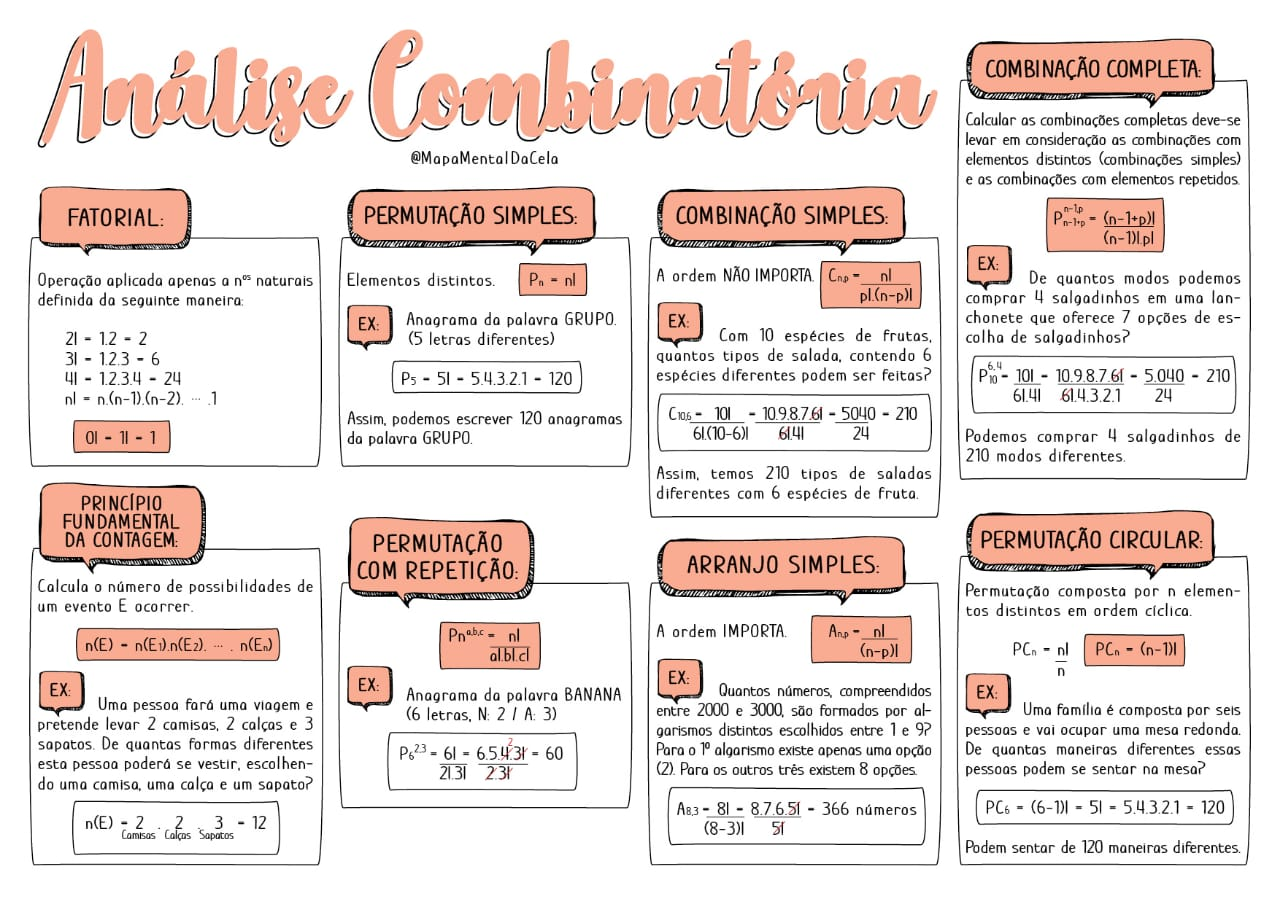
\includegraphics[scale=0.35]{../../imagens/mapa-mental-analise-combinatoria.jpeg}
\label{mapa-mental-analise-combinatoria}
Fonte:\href{https://infinittusexatas.com.br/analise-combinatoria-resumos-e-mapas-mentais/}{Site Infinittus - Conhecimento nas medidas exatas}
\end{figure}

\section{Exercícios Resolvidos}

\begin{enumerate}

\item[\textbf{R1}] Uma montadora de automóveis apresenta um carro em \textbf{quatro modelos} diferentes e em \textbf{cinco cores} diferentes. Um consumidor que quiser arquirir esse veículo terá quantas opções de escolha ?

  \begin{itemize}
    \item[\ding{172}] \textbf{O que contar?:} Quantas opções de escolha de veículo o consumidor terá ?
    \item[\ding{173}] \textbf{Restrições do(s) Experimento(s):} Nenhuma.
    \item[\ding{174}] \textbf{Experimento 1:} Escolher uma das opções de modelo. $n_{1}$ possui 5 resultados possíveis.
    \item[\ding{175}] \textbf{Experimento 2:} Escolher uma das opções de cor. $n_{2}$ possui 4 resultados possíveis.
    \item[\ding{176}] \textbf{Cálculo:} Pelo princípio fundamental da contagem (PFC), o experimento composto 1 e 2, nessa ordem, tem $n_{1} \times n_{2}$ resultados possíveis, ou seja, $5 \times 4 = 20$ opções de escolha.
    \item[\ding{177}] \textbf{Conclusão:}  existem 20 opções de escolha de veículos para o consumidor.
  \end{itemize}
  
  \newpage

\item[\textbf{R2}] Quantos números naturais de três algarismos podem ser formados com os algarismos $A = \{1, 2, 6, 8, 9\}$ ?
   \begin{itemize}
    \item[\ding{172}] \textbf{O que contar?:} Quantos números naturais de três algarismos podem ser formados com os algarismos dados.
    \item[\ding{173}] \textbf{Restrições do(s) Experimento(s):} Nenhuma.
    \item[\ding{174}] \textbf{Experimento 1:} $E_1$ = Preencher a posição das unidades com um dos algarismos dados.\\ Sendo $n_{1}$ o número de resultados possíveis do \textbf{experimento 1}, $n_{1}$ possui $n(A)$ resultados possíveis, ou seja, $n_{1} = n(A) = 5$.
    
    \item[\ding{175}] \textbf{Experimento 2:} $E_2$ = Preencher a posição das dezenas com um dos algarismos dados.\\ Sendo $n_{2}$ o número de resultados possíveis do \textbf{experimento 2}, $n_{2}$ possui $n(A)$ resultados possíveis, já que nenhuma restrição existe para realizarmos o experimento, ou seja, $n_{2} = n(A) = 5$.
    
    \item[\ding{176}] \textbf{Experimento 2:} $E_3$ = Preencher a posição das centenas com um dos algarismos dados.\\ Sendo $n_{1}$ o número de resultados possíveis do \textbf{experimento 2}, $n_{3}$ possui $n(A)$ resultados possíveis, já que nenhuma restrição existe para realizarmos o experimento, ou seja, $n_{3} = n(A) = 5$.
    
    \item[\ding{177}] \textbf{Cálculo:} Pelo princípio fundamental da contagem (PFC), os experimentos 1, 2 e 3 apresentam, respectivamente, $n_{1},\, n_{2} \textrm{ e } n_{3}$ resultados possíveis, logo o experimento composto 1, 2 e 3 possuem, nessa ordem, $n_{1} \times n_{2} \times n_{3}$ ou $5 \times 5 \times 5 = 125$ resultados possíveis.
    \item[\ding{178}] \textbf{Conclusão:} Podemos formar \textbf{125 números naturais de três algarismos} com os números dados.
 \end{itemize}
  
\item[\textbf{R3}] Quantos números naturais de três algarismos \textbf{distintos} podem ser formados com os algarismos $A = \{1, 2, 6, 8, 9\}$ ?
   \begin{itemize}
    \item[\ding{172}] \textbf{O que contar?:} Quantos números naturais de três algarismos \textbf{distintos} podem ser formados com os algarismos dados.
    \item[\ding{173}] \textbf{Restrições do(s) Experimento(s):} Os números escolhidos em cada experimento devem ser distintos.
    \item[\ding{174}] \textbf{Experimento 1:} $E_1$ = Preencher a posição das unidades com um dos algarismos dados.\\ Sendo $n_{1}$ o número de resultados possíveis do \textbf{experimento 1}, $n_{1}$ possui $n(A)$ resultados possíveis, ou seja, $n_{1} = n(A) = 5$.
    \item[\ding{175}] \textbf{Experimento 2:} $E_2$ = Preencher a posição das dezenas com um dos algarismos dados.\\ Sendo $n_{2}$ o número de resultados possíveis do \textbf{experimento 2}, $n_{2}$ possui $n(A)-1$ resultados possíveis,pois um dos algarismos já foi escolhido no experimento 1, ou seja, $n_{2} = n(A)-1 = 5 - 1 = 4$.
    \item[\ding{176}] \textbf{Experimento 3:} $E_3$ = Preencher a posição das centenas com um dos algarismos dados.\\ Sendo $n_{3}$ o número de resultados possíveis do \textbf{experimento 3}, $n_{3}$ possui $n(A)-2$ resultados possíveis,pois um dos algarismos já foi escolhido no \textbf{experimento 1} e outro no \textbf{experimento 2}, ou seja, $n_{2} = n(A) - 2 = 5 - 2 = 3$.   
    \item[\ding{177}] \textbf{Cálculo:} Pelo princípio fundamental da contagem (PFC), os experimentos 1, 2 e 3 apresentam, respectivamente, $n_{1},\, n_{2} \textrm{ e } n_{3}$ resultados possíveis, logo o experimento composto 1, 2 e 3 possuem, nessa ordem, $n_{1} \times n_{2} \times n_{3}$ ou $5 \times 4 \times 3 = 60$ resultados possíveis.
    \item[\ding{178}] \textbf{Conclusão:} Podemos formar \textbf{60 números naturais de três algarismos distintos} com os números dados.
  \end{itemize}
  
\item[\textbf{R4}] Quantos números naturais de três algarismos \textbf{distintos} podem ser formados com os algarismos $A = \{0, 1, 2, 6, 8\}$ ?
   \begin{itemize}
    \item[\ding{172}] \textbf{O que contar?:} Quantos números naturais de três algarismos \textbf{distintos} podem ser formados com os algarismos dados.
    
    \item[\ding{173}] \textbf{Restrições do(s) Experimento(s):}
      \begin{enumerate}
    		\item[a)] Os números escolhidos em cada experimento devem ser distintos.
    		\item[b)] A posição da \textbf{centena} não pode conter o número zero ( 0 ), pois, nesse caso, o número natural formado não terá três algarismos, e sim dois.
      \end{enumerate}
    \item[\ding{174}] \textbf{Experimento 1:} $E_1$ = Preencher a posição das centenas com um dos algarismos dados, observando as duas restrições apontadas do experimento.\\ Lembrando que o zero não pode ser excolhido. Sendo $n_{1}$ o número de resultados possíveis do \textbf{experimento 1}, $n_{1}$ possui $n(A)$ resultados possíveis, ou seja, $n_{1} = n(A)-1 = 4$.
    
    \item[\ding{175}] \textbf{Experimento 2:} $E_2$ = Preencher a posição das dezenas com um dos algarismos dados, observando as duas restrições apontadas do experimento.\\ Lembrando que: (1) Já foi escolhido o algarismo das centenas e (2) para casa das dezenas o zero pode ser escolhido.\\ Sendo $n_{2}$ o número de resultados possíveis do \textbf{experimento 2}, $n_{2}$ possui $n(A)-1$ resultados possíveis,pois um dos algarismos já foi escolhido no experimento 1 e o zero pode ser escolhido, ou seja, $n_{2} = n(A)-1 = 5 - 1 = 4$.
    
    \item[\ding{176}] \textbf{Experimento 3:} $E_2$ = Preencher a posição das unidades com um dos algarismos dados, observando as duas restrições apontadas do experimento.\\ Lembrando que: (1) Já foi escolhido o algarismo das centenas e das dezenas e (2) para casa das unidades o zero pode ser escolhido.\\ Sendo $n_{2}$ o número de resultados possíveis do \textbf{experimento 2}, $n_{2}$ possui $n(A)-2$ resultados possíveis,pois um dos algarismos já foi escolhido no experimento 1, outro algarismo no experimento 2 e o zero pode ser escolhido, ou seja, $n_{2} = n(A)-2 = 5 - 2 = 3$.
      
    \item[\ding{177}] \textbf{Cálculo:} Pelo princípio fundamental da contagem (PFC), os experimentos 1, 2 e 3 apresentam, respectivamente, $n_{1},\, n_{2} \textrm{ e } n_{3}$ resultados possíveis, logo o experimento composto 1, 2 e 3 possuem, nessa ordem, $n_{1} \times n_{2} \times n_{3}$ ou $4 \times 4 \times 3 = 48$ resultados possíveis.
    
    \item[\ding{178}] \textbf{Conclusão:} Podemos formar \textbf{48 números naturais de três algarismos distintos} com os números dados.
  \end{itemize}
  
\item[\textbf{R5}] Quantos divisores naturais possui o número 72?
   \begin{itemize}
    \item[\ding{172}] \textbf{O que contar?} Quantos divisores naturais possui o número 72.
    
    \item[\ding{173}] \textbf{Restrições do(s) Experimento(s):} Nenhum.

    \item[\ding{174}] Fatoramos o número 72.
    
      \begin{table}[H]
        \centering
        Fatoração do número 72 \\
        \begin{tabular}{c|c}
     	  72 & 2 \\
	      36 & 2 \\
          18 & 2 \\
          9 & 3 \\          
          3 & 3 \\ \hline
          1 & $2^4 \cdot 3^2$ \\     
       \end{tabular}
       \label{fatoracao-numero-72}       
     \end{table}

    
    \item[\ding{175}] A partir da fatoração realizada no item 3, podemos construir uma lista de divisores do número 72. Qualquer número que pode ser escrito através do produto $2^{\{0..3\}} \times 3^{\{0..2\}} $, com $x \in \{0,1,2,3\}$ e $y \in \{0,1,2\}$, é um divisor de 72. Ou seja, os divisores são: 

      \begin{center}
     	$D(72)=\{2^0 \times 3^0,
     	2^0 \times 3^0,
     	2^0 \times 3^1,
     	2^0 \times 3^2,
     	2^1 \times 3^0,
     	2^1 \times 3^1,
     	2^1 \times 3^2,
     	2^2 \times 3^0,
     	2^2 \times 3^1,
     	2^2 \times 3^2,
     	2^3 \times 3^0,
     	2^3 \times 3^1,
     	2^3 \times 3^2
     	\}$ \\
     	ou \\
     	$D(72)=\{
        1,2,3,4,6,
        8,9,12,18,24,
        36,72\}
     	$
     \end{center}
        
    Um outra forma, mais genérica e rápida, de constatar que 72 possui 12 divisores é descobrir de quantas maneiras, no produto $2^{\{0..3\}} \times 3^{\{0..2\}} $, com $x \in \{0,1,2,3\}$ e $y \in \{0,1,2\}$, eu posso preencher o expoente do 2 e o expoente do 3. \\Percebe-se que, tal qual respondemos nas questões anteriores, pelo princípio fundamental da contagem (PFC), temos dois experimentos: $E_1 =$ Preencher o expoente do 2 e $E_2 =$ Preencher o expoente do 3. Sendo $n_{1}$ o número de resultados possíveis do experimento $E_1$ e $n_{2}$ o número de resultados possíveis do experimento $E_2$, temos que pelo PFC, o experimento composto $E_1$ e $E_2$, nessa ordem, apresenta $n_{1} \times n_{2}$ resultados possíveis, ou seja $4 \times 3 = 12$ números (divisores).
       
    \item[\ding{178}] \textbf{Conclusão:} O número 72 possui \textbf{12 divisores naturais}.
  \end{itemize}
  
\item[\textbf{R6}] Quantos subconjuntos possui o conjunto $A = \{a,b,c,d\}$?

    \begin{figure}[htb]
      \centering
      \caption{[Questão R6, pág.158] - Os elementos dos subconjuntos do conjunto A}
      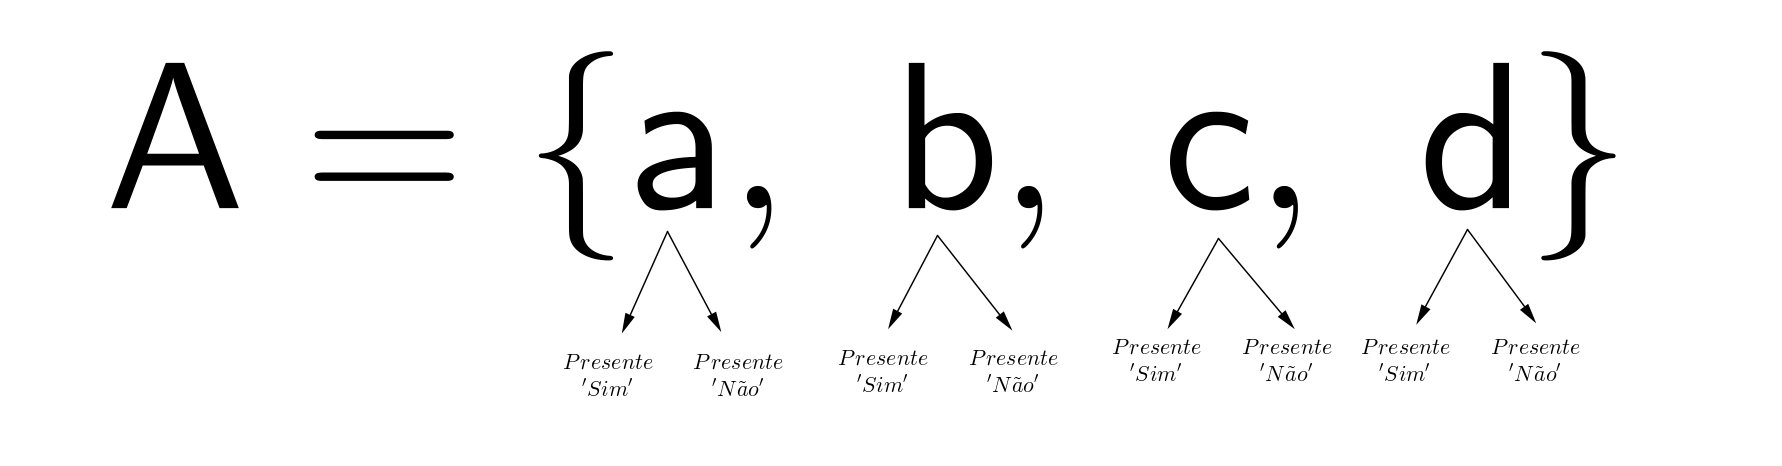
\includegraphics[scale=0.8]{../../imagens/geogebra-cap21-exercicios-R6-pag158.png}
      \caption*{Fonte: Autor}
      \label{geogebra-cap21-exercicios-R6-pag158}
    \end{figure}


   \begin{itemize}
    \item[\ding{172}] \textbf{O que contar?:} Quantos subconjuntos possui o conjunto A.
    
    \item[\ding{173}] \textbf{Restrições do(s) Experimento(s):} Nenhum.
    
    \item[\ding{174}] \textbf{Experimento:} trata-se de um experimento composto de vários experimentos, conforme explicitamos abaixo.
      \begin{itemize}
          \item[\ding{172}] \textbf{$E_1$} Escolher se o \textbf{1º} elemento do conjunto de A, "a", será ou não escolhido. Esse experimento possui $n(E_1) = 2$ resultados possíveis (presente ou não presente).
          \item[\ding{173}] \textbf{$E_1$} Escolher se o \textbf{2º} elemento do conjunto de A, "b", será ou não escolhido. Esse experimento possui $n(E_2) = 2$ resultados possíveis (presente ou não presente)
          \item[\ding{174}] \textbf{$E_1$} Escolher se o \textbf{3º} elemento do conjunto de A, "c", será ou não escolhido. Esse experimento possui $n(E_3) = 2$ resultados possíveis (presente ou não presente)
          \item[\ding{175}] \textbf{$E_1$} Escolher se o \textbf{4º} elemento do conjunto de A, "d", será ou não escolhido. Esse experimento possui $n(E_4) = 2$ resultados possíveis (presente ou não presente)
      \end{itemize}
    
    \item[\ding{175}] \textbf{Cálculo:} Pelo princípio fundamental da contagem (PFC), os experimentos 1, 2, 3 e 4 apresentam, respectivamente, $n_{1},\, n_{2},\, n_{3} \textrm{ e } n_{4}$ resultados possíveis, logo o experimento composto 1, 2, 3 e 4 possuem, nessa ordem, $n_{1} \times n_{2} \times n_{3} \times n_{4}$ ou $2 \times 2 \times 2 \times 2 = 16$ resultados possíveis.
    
    \item[\ding{178}] \textbf{Conclusão:} Podemos formar \textbf{16 subconjuntos de A, incluindo o conjunto vazio}.
    
  \end{itemize}

\end{enumerate}

\section{Exercícios Básicos}

\begin{enumerate}

\item[\textbf{B1}] Duas linhas de ônibus vão de uma cidade A para uma cidade B e três linhas vão da cidade B para uma cidade C. De quantos modos diferentes um usuário dessas linhas pode ir de A para C, passando por B ?

    \begin{figure}[htb]
      \centering
      \caption{[Questão B1, pág.159] - Esquema das opções de transporte de A para C, passando por B}
      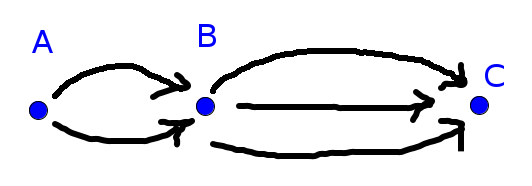
\includegraphics[scale=0.6]{../../imagens/geogebra-cap21-exercicios-B1-pag159.png}
      \caption*{Fonte: Autor}
      \label{geogebra-cap21-exercicios-B1-pag159}
    \end{figure}

   \begin{itemize}
     \item[\ding{172}] \textbf{Experimento 1:} $E_1$ = Escolher uma das duas linhas de ônibus de A para B. Esse experimento possui $n(E_1) = 2$ resultados possíveis.
     \item[\ding{173}] \textbf{Experimento 2:} $E_2$ = Escolher uma das três linhas de ônibus de B para C. Esse experimento possui $n(E_2) = 3$ resultados possíveis.
     \item[\ding{174}] \textbf{Cálculo:} Pelo princípio fundamental da contagem (PFC), os experimentos 1 e 2 apresentam, respectivamente, $n_{1} \textrm{ e } n_{2}$ resultados possíveis, logo o experimento composto 1 e 2 possui, nessa ordem, $n_{1} \times n_{2}$ ou $2 \times 3 = 6$ resultados possíveis.
     \item[\ding{175}] \textbf{Conclusão:} O usuário dessas linhas pode ir de A para C, passando por B, de \textbf{6 formas diferentes}.   \end{itemize}
  
\item[\textbf{B2}] Quantos números naturais \textbf{de quatro algarismos} podem ser formados com os algarismos 3, 4, 5, 6, 7, 8 e 9?
 \begin{itemize}
     \item[\ding{172}] \textbf{Experimento 1:} $E_1$ = Escolher o algarismo da \textbf{unidade de milhar} dentre os algarismos dados. Esse experimento possui $n(E_1) = 7$ resultados possíveis.
     \item[\ding{173}] \textbf{Experimento 2:} $E_2$ = Escolher o algarismo da \textbf{centena} dentre os algarismos dados. Esse experimento possui $n(E_2) = 7$ resultados possíveis.
     \item[\ding{174}] \textbf{Experimento 3:} $E_3$ = Escolher o algarismo da \textbf{dezena} dentre os algarismos dados. Esse experimento possui $n(E_3) = 7$ resultados possíveis.
     \item[\ding{175}] \textbf{Experimento 4:} $E_4$ = Escolher o algarismo da \textbf{unidade} dentre os algarismos dados. Esse experimento possui $n(E_4) = 7$ resultados possíveis.    
     \item[\ding{176}] \textbf{Cálculo:} Pelo princípio fundamental da contagem (PFC), os experimentos 1, 2, 3 e 4 apresentam, respectivamente, $n_{1}, n_{2}, n_{3} \textrm{ e } n_{4}$ resultados possíveis, logo o experimento composto 1, 2, 3 e 4 possui, nessa ordem, $n_{1} \times n_{2} \times n_{3} \times n_{4}$ ou $7 \times 7 \times 7 \times 7 = 2401$ resultados possíveis.
     \item[\ding{177}] \textbf{Conclusão:} \textbf{2.401 números naturais de quatro algarismos} podem ser formados com os algarismos 3, 4, 5, 6, 7, 8 e 9. 
   \end{itemize}

\item[\textbf{B3}] Quantos números naturais de \textbf{quatro algarismos distintos} podem ser formados com os algarismos 3, 4, 5, 6, 7, 8 e 9?
 \begin{itemize}
     \item[\ding{172}] \textbf{Restrição do(s) Experimento(s):} Os algarismos dos números naturais formados \textbf{devem ser distintos}.
     \item[\ding{173}] \textbf{Experimento 1:} $E_1$ = Escolher o algarismo da \textbf{unidade de milhar} dentre os algarismos dados. Esse experimento possui $n(E_1) = 7$ resultados possíveis.
     \item[\ding{174}] \textbf{Experimento 2:} $E_2$ = Escolher o algarismo da \textbf{centena} dentre os algarismos dados, sem contar o que foi escolhido no experimento 1($E_1$). Esse experimento possui $n(E_2) = 7 - 1 = 6$ resultados possíveis.
     \item[\ding{175}] \textbf{Experimento 3:} $E_3$ = Escolher o algarismo da \textbf{dezena} dentre os algarismos dados, sem contar o que foi escolhido nos experimentos 1 e 2 ($E_1 \textrm{ e }E_2$). Esse experimento possui $n(E_3) = 7 - 2 = 5$ resultados possíveis.
     \item[\ding{176}] \textbf{Experimento 4:} $E_4$ = Escolher o algarismo da \textbf{unidade} dentre os algarismos dados, sem contar o que foi escolhido nos experimentos 1, 2 e 3 ($E_1 \textrm{ e } E_2 \textrm{ e } E_3$). Esse experimento possui $n(E_4) = 7 - 3 = 4$ resultados possíveis.    
     \item[\ding{177}] \textbf{Cálculo:} Pelo princípio fundamental da contagem (PFC), os experimentos 1, 2, 3 e 4 apresentam, respectivamente, $n_{1}, n_{2}, n_{3} \textrm{ e } n_{4}$ resultados possíveis, logo o experimento composto 1, 2, 3 e 4 possui, nessa ordem, $n_{1} \times n_{2} \times n_{3} \times n_{4}$ ou $7 \times 6 \times 5 \times 4 = 840$ resultados possíveis.
     \item[\ding{178}] \textbf{Conclusão:} \textbf{840 números naturais de quatro algarismos distintos} podem ser formados com os algarismos 3, 4, 5, 6, 7, 8 e 9. 
   \end{itemize}

\item[\textbf{B4}] Quantos números naturais de \textbf{cinco algarismos distintos} podem ser formados com os algarismos $A = \{0, 3, 4, 5, 6, 7, 8, 9\}$?
 \begin{itemize}
     \item[\ding{172}] \textbf{Dados para o Problema:} O número de elementos de A é dado pela expressão: $n(A)= 8$.
     \item[\ding{173}] \textbf{Restrições do(s) Experimento(s):}
        \begin{enumerate}[a)]
          \item Os algarismos dos números naturais formados \textbf{devem ser distintos};
          \item A escolha do algarismo da \textbf{dezena de milhar} não pode ser zero, pois, nesse caso, o número natural formado não terá \textbf{cinco algarismos}.
        \end{enumerate}
     \item[\ding{174}] \textbf{Experimento 1:} $E_1$ = Escolher o algarismo da \textbf{dezena de milhar}, exceto o zero, dentre os algarismos dados. Esse experimento possui $n(E_1) = n(A) - 1 = 8 - 1 = 7$ resultados possíveis.
     \item[\ding{175}] \textbf{Experimento 2:} $E_2$ = Escolher o algarismo da \textbf{centena} dentre os algarismos dados, sem contar o que foi escolhido no experimento 1($E_2$) e considerando que o zero pode ser escolhido. Esse experimento possui $n(E_2) = n(A) - 1 = 8 - 1 = 7$ resultados possíveis.
     \item[\ding{175}] \textbf{Experimento 3:} $E_3$ = Escolher o algarismo da \textbf{centena} dentre os algarismos dados, sem contar o que foi escolhido no experimento 1 e 2 ($E_1 \textrm{ e } E_2$) e considerando que o zero pode ser escolhido. Esse experimento possui $n(E_3) = n(A) - 2 = 8 - 2 = 6$ resultados possíveis.     
     \item[\ding{175}] \textbf{Experimento 4:} $E_4$ = Escolher o algarismo da \textbf{centena} dentre os algarismos dados, sem contar o que foi escolhido no experimento 1, 2 e 3 ($E_1 \textrm{ e } E_2 \textrm{ e } E_3$) e considerando que o zero pode ser escolhido. Esse experimento possui $n(E_4) = n(A) - 3 = 8 - 3 = 5$ resultados possíveis.
     \item[\ding{175}] \textbf{Experimento 5:} $E_5$ = Escolher o algarismo da \textbf{centena} dentre os algarismos dados, sem contar o que foi escolhido no experimento 1, 2, 3 e 4 ($E_1 \textrm{ e } E_2 \textrm{ e } E_3 \textrm{ e } E_4$) e considerando que o zero pode ser escolhido. Esse experimento possui $n(E_5) = n(A) - 4 = 8 - 4 = 4$ resultados possíveis.       
     \item[\ding{178}] \textbf{Cálculo:} Pelo princípio fundamental da contagem (PFC), os experimentos 1, 2, 3, 4 e 5 apresentam, respectivamente, $n_{1}, n_{2}, n_{3}, n_{4} \textrm{ e } n_{5}$ resultados possíveis, logo o experimento composto 1, 2, 3, 4 e 5 possui, nessa ordem, $n_{1} \times n_{2} \times n_{3} \times n_{4} \times n_{5}$ ou $7 \times 7 \times 6 \times 5 \times 4 = 5880$ resultados possíveis.
     \item[\ding{179}] \textbf{Conclusão:} \textbf{5880 números naturais de cinco algarismos distintos} podem ser formados com os algarismos 0, 3, 4, 5, 6, 7, 8, 9. 
   \end{itemize}

\item[\textbf{B5}] Quantos números pares e positivos de três algarismos distintos podem ser formados com os algarismos 3, 4, 5, 6, 7, 8 e 9?
 \begin{itemize}
     \item[\ding{172}] \textbf{Dados para o problema:} O número de elementos de A é dado pela expressão: $n(A)= 7$.
     \item[\ding{173}] \textbf{Restrições do(s) Experimento(s):}
        \begin{enumerate}[a)]
          \item Devemos formar números naturais de três algarismos \textbf{distintos};
          \item Os algarismos das unidades deve ser par, dentre os algarismos disponíveis, ou seja, $4, 6 \textrm{ ou } 8$;          
        \end{enumerate}
     \item[\ding{174}] \textbf{Experimento 1:} $E_1$ = Escolher o algarismo das \textbf{unidades}, dentre os algarismos dados de forma que o número seja par, ou seja, escolher entre $4, 6 \textrm{ ou } 8$. Esse experimento possui $n(E_1) = 3$ resultados possíveis.
     \item[\ding{175}] \textbf{Experimento 2:} $E_2$ = Escolher o algarismo da \textbf{dezenas} dentre os algarismos dados, sem contar o que foi escolhido no experimento 1($E_1$) e considerando a restrição "a" (algarismos distintos). Esse experimento possui $n(E_2) = n(A) - 1 = 6$ resultados possíveis.
     \item[\ding{176}] \textbf{Experimento 3:} $E_3$ = Escolher o algarismo da \textbf{centena} dentre os algarismos dados, sem contar o que foi escolhido no experimento 1 e 2 ($E_1 \textrm{ e } E_2$) e considerando a restrição "a" (algarismos distintos). Esse experimento possui $n(E_2) = n(A) - 2 = 5$ resultados possíveis.
     \item[\ding{177}] \textbf{Cálculo:} Pelo princípio fundamental da contagem (PFC), os experimentos 1, 2 e 3 apresentam, respectivamente, $n_{1}, n_{2} \textrm{ e } n_{3}$ resultados possíveis, logo o experimento composto 1, 2 e 3 possui, nessa ordem, $n_{1} \times n_{2} \times n_{3}$ ou $3 \times 6 \times 5 = 90$ resultados possíveis.
     \item[\ding{178}] \textbf{Conclusão:} \textbf{90 números pares positivos de três algarismos distintos} podem ser formados com os algarismos 3, 4, 5, 6, 7, 8 e 9. 
   \end{itemize}

\item[\textbf{B6}] Quatro linhas de ónibus unem a cidade A à cidade B e três linhas unem a cidade B à cidade C. Um usuário vai viajar de A para C passando por B e vai voltar para A, passando novamente por B. De quantos modos diferentes esse usuário poderá escolher as linhas, se na volta ele não puder usar a linha que usou na ida? 

 \begin{itemize}
     \item[\ding{172}] \textbf{Restrições do(s) Experimento(s):}
        \begin{enumerate}[a)]
          \item Ir de A para C, passando por B;
          \item Voltar de C para A, passando por B e \textbf{não utilizando os ônibus usados na IDA de A para C};
        \end{enumerate}
     \item[\ding{173}] \textbf{Experimento 1:} $E_1$ = Escolher o ônibus para ir da A para B. Esse experimento possui $n(E_1) = 4$ resultados possíveis.
     \item[\ding{174}] \textbf{Experimento 2:} $E_2$ = Escolher o ônibus para ir da B para C. Esse experimento possui $n(E_2) = 3$ resultados possíveis.
     \item[\ding{175}] \textbf{Experimento 3:} $E_3$ = Escolher o ônibus para ir da C para B, \textbf{não podendo escolher o que foi utilizado no experimento 2 ($E_2$)}. Esse experimento possui $n(E_3) = 3 - 1 = 2$ resultados possíveis.
     \item[\ding{176}] \textbf{Experimento 4:} $E_4$ = Escolher o ônibus para ir da B para A, \textbf{não podendo escolher o que foi utilizado no experimento 1 ($E_1$)}. Esse experimento possui $n(E_4) = 4 - 1 = 3$ resultados possíveis.    
     \item[\ding{177}] \textbf{Cálculo:} Pelo princípio fundamental da contagem (PFC), os experimentos 1, 2, 3 e 4 apresentam, respectivamente, $n_{1}, n_{2}, n_{3} \textrm{ e } n_{4}$ resultados possíveis, logo o experimento composto 1, 2, 3 e 4 possui, nessa ordem, $n_{1} \times n_{2} \times n_{3} \times n_{4}$ ou $4 \times 3 \times 2 \times 3 = 72$ resultados possíveis.
     \item[\ding{178}] \textbf{Conclusão:} Para fazer a viagem de IDA e VOLTA conforme especificado no enunciado da questão, existem \textbf{72 possibilidade distintas}.
   \end{itemize}

\item[\textbf{B7}] Oito atletas participam de uma corrida. Serão premiados apenas os três primeiros lugares. De quantas maneiras diferentes os prêmios podem ser distribuídos?
 \begin{itemize}
     \item[\ding{172}] \textbf{Dados para o problema:}
        \begin{enumerate}[a)]
          \item O número de atletas que participam da corrida é dado pela expressão: $n(A)= 8$;
          \item Serão premiados apenas os \textbf{três primeiros lugares};          
        \end{enumerate}     
     \item[\ding{173}] \textbf{O que se dejesa saber?}
        \begin{enumerate}[a)]
          \item De quantas maneiras diferentes os prêmios podem ser distribuídos?
        \end{enumerate}
     \item[\ding{174}] \textbf{Experimento 1:} $E_1$ = Premiar o corredor que terminou em \textbf{primeiro} lugar. Esse experimento possui $n(E_1) =n(A) = 8$ resultados possíveis.
     \item[\ding{175}] \textbf{Experimento 2:} $E_2$ = Premiar o corredor que terminou em \textbf{segundo lugar}. Esse experimento possui $n(E_2) =n(A) - 1 = 8 - 1 = 7$ resultados possíveis já que desconsideramos o corredor que terminou em 1º lugar.
     \item[\ding{176}] \textbf{Experimento 3:} $E_3$ = Premiar o corredor que terminou em \textbf{terceiro lugar}. Esse experimento possui $n(E_3) =n(A) - 2 = 8$ resultados possíveis já que desconsideramos o corredor que terminou em 1º e em 2º lugar.
     \item[\ding{177}] \textbf{Cálculo:} Pelo princípio fundamental da contagem (PFC), os experimentos 1, 2 e 3 apresentam, respectivamente, $n_{1}, n_{2} \textrm{ e } n_{3}$ resultados possíveis, logo o experimento composto 1, 2 e 3 possui, nessa ordem, $n_{1} \times n_{2} \times n_{3}$ ou $8 \times 7 \times 6 = 336$ resultados possíveis.
     \item[\ding{178}] \textbf{Conclusão:} Os prêmios podem ser distribuídos de \textbf{336 maneiras diferentes}.
   \end{itemize}

\item[\textbf{B8}] Uma prova é constituída por dez testes do tipo "verdadeiro ou falso". De quantas maneiras diferentes um candidato poderá responder aos dez testes, não deixando nenhum sem resposta e assinalando apenas uma alternativa em cada um?
  \begin{itemize}
    \item[\ding{172}] \textbf{O que contar?:} Tratam-se de dez experimentos, um para cada questão, que consistem em escolher a ALTERNATIVA "V" OU "F", havendo, portanto, dois resultados possíveis para cada experimento.
    \item[\ding{173}] \textbf{Restrições do(s) Experimento(s):} Ao responder as questões, o candidato:
        \begin{enumerate}[a)]
          \item Não pode deixar nenhuma questão sem resposta
          \item Deve asinalar apenas uma alternativa em cada questão ("V" ou "F")
        \end{enumerate}     
    \item[\ding{174}] \textbf{Experimentos:} Em síntese, tratam-se de dez experimentos, um para cada questão, que consistem em escolher a alternativa "V" OU "F", ou seja $n(A_n) = 2$ para cada experimento.
    \item[\ding{175}] \textbf{Cálculo:} Pelo princípio fundamental da contagem (PFC), os experimentos 1, 2, 3, ..., 10 apresentam, respectivamente, $n_{1},\, n_{2},\, n_{3} \textrm{, ..., } n_{10}$ resultados possíveis, logo o experimento composto 1, 2, 3, ..., 10 possuem, nessa ordem, $n_{1} \times n_{2} \times n_{3} \times \textrm{ ... } \times n_{4}$ ou $2 \times 2 \times 2  \times \textrm{ ... }  \times 2 = 2^{10} = 1024$ resultados possíveis. 
    \item[\ding{176}] \textbf{Conclusão:} A prova poderá ser respondida de \textbf{1024 maneiras distintas}.  
  \end{itemize}

\item[\textbf{B9}] Quantos números de telefone de seis dígitos podem ser formados com os dígitos 1, 2, 3, 4, 5, 6 e 7, de modo que os três primeiros dígitos sejam distintos?
  \begin{itemize}
    \item[\ding{172}] \textbf{O que contar?:} Tratam-se de 6 experimentos, escolher cada um dos algarismos de telefone a ser formado, respeitando as restrições abaixo.
    \item[\ding{173}] \textbf{Restrições do(s) Experimento(s):}
        \begin{enumerate}[a)]
          \item Os três primeiros algarismos do número de telefone devem ser distintos.
        \end{enumerate}     

   \begin{figure}[htb]
      \centering
      \caption{[Questão B9, pág.159] - Esquema - Quantos números podemos formar?}
      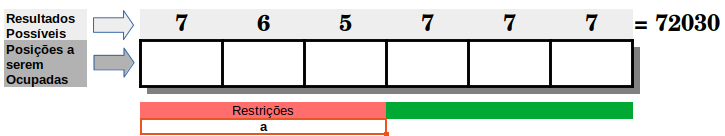
\includegraphics[scale=0.6]{../../imagens/cap21-exercicios-B9-pag159.png}
      \caption*{Fonte: Autor}
      \label{cap21-exercicios-B9-pag159}
    \end{figure}
    
    \item[\ding{174}] \textbf{Experimentos:} Em síntese, tratam-se de seis experimentos: Escolher um algarismo dentre os dígitos 1, 2, 3, 4, 5, 6 e 7.
    \item[\ding{175}] \textbf{Cálculo:} 
    
		\begin{itemize}[a)]
		  \item Atuamos primeiro nos três primeiros algarismos que possuem restrições. A primeira posição pode ser ocupada por 7 dos disgitos disponíveis. A segunda possição poderá ser ocupada por 6 algarismos($7-1$), a terceira por 5 ($7-2$), já que eles devem ser distintos (restrição "a").
		  \item As demais posições do número de telefone não possuem restrição. Elas podem receber quaisquer dos dígitos 1, 2, 3, 4, 5, 6 e 7, disponíveis.		  
		\end{itemize}
   \item[\ding{176}] Pelo princípio fundamental da contagem (PFC), as posições podem ser preenchidas conforme a figura \ref{cap21-exercicios-B9-pag159}.
   \item[\ding{177}] \textbf{Conclusão:} Podem ser formados \textbf{72.030 telefones diferentes} obedecendo os critérios do enunciado da questão.  
  \end{itemize}

\newpage

\item[\textbf{B10}] Uma placa de automóvel é formada por três letras seguidas de quatro algarismos, por exemplo: "BNP - 0339". Quantas placas podem ser formadas com pelo menos um algarismo não-nulo, dispondo-se das 26 letras do alfabeto e dos dez algarismos do sistema decimal? (Incluímos as letras Y, W e K.) 
  \begin{itemize}
    \item[\ding{172}] \textbf{O que contar?:} Tratam-se de 2 experimentos. $E_1 =$ Escolher três as letras para a placa do automóvel. $E_2 =$ Escolher 4 números para a placa, respeitando as restrições do enunciado da questão.
    \item[\ding{173}] \textbf{Restrições do(s) Experimento(s):}
        \begin{enumerate}[a)]
          \item A parte numérica da placa deve conter, \textbf{pelo menos} um algarismo não-nulo (1,2,3,4,5,6,7,8 e 9), ou seja, existem três situações distintas que devem ser tratadas: A parte numérica da placa deve conter três algarismos zero, dois algarismos zero ou um algarismo zero, \textbf{mas não os quatro algarismos zero}.
        \end{enumerate}  
   \begin{figure}[!htb]
      \centering
      \caption{[Questão B10, pág.159] - Formar placas com \textbf{pelo menos um} dígito não-nulo.}
      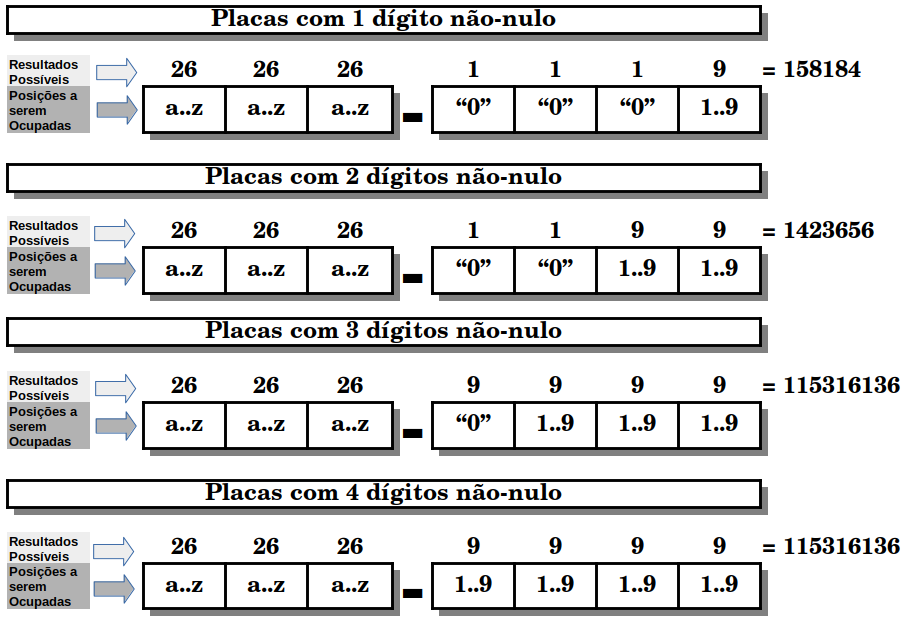
\includegraphics[scale=0.5]{../../imagens/cap21-exercicios-B10-pag159.png}
      \caption*{Fonte: Autor}
      \label{cap21-exercicios-10-pag159}
    \end{figure}
    
  \end{itemize}
  
\newpage
  
\item[\textbf{B11}] Qual o número de divisores naturais de $n = 2^4 \times 3^3 \times 5$?
  \begin{itemize}
    \item[\ding{172}] \textbf{O que contar?} A partir da fatoração $ 2^4 \times 3^3 \times 5 = 2160 $, podemos construir uma lista de divisores possíveis. Qualquer número que pode ser escrito através do produto $2^x \times 3^y \times 5^z$ , com $x \in \{0,1,2,3,4\}$ , $y \in \{0,1,2,3\}$ e $z \in \{0,1\}$, é um divisor de 2160, ou seja, se dividirmos o número $2160 \textrm{ por } 2^x \times 3^y \times 5^z$ ocorrerá divisão exata (com resto zero). Em resumo, qualquer número $b, b \in \mathbb{N}$, será divisor de um número $a, a \in \mathbb{N}$, se na divisão $\dfrac{a}{b}$, o resto for zero.
    \item[\ding{173}] \textbf{Experimento 1:} $E_1$ = Escolher o expoente para o \textbf{fator 2} em $2^x \times 3^y \times 5^z$. Com $x \in \{0,1,2,3,4\}$, esse experimento possui $n(E_1) = n_1 = 5$ resultados possíveis.
    \item[\ding{174}] \textbf{Experimento 2:} $E_2$ = Escolher o expoente para o \textbf{fator 3} em $2^x \times 3^y \times 5^z$. Com $y \in \{0,1,2,3\}$ , esse experimento possui $n(E_2) = n_2 = 4$ resultados possíveis.
    \item[\ding{175}] \textbf{Experimento 3:} $E_3$ = Escolher o expoente para o \textbf{fator 5} em $2^x \times 3^y \times 5^z$. Com $z \in \{0,1\}$, esse experimento possui $n(E_3) = n_3 = 2$ resultados possíveis.
    \item[\ding{176}] \textbf{Cálculo:} Pelo princípio fundamental da contagem (PFC), o experimento $E_1$ possui $n_1$ resultados possíveis, o experimento $E_2$ possui $n_2$ resultados possíveis e o experimento $E_3$ possui $n_3$ resultados possíveis, logo o experimento composto $E_1, E_2 \textrm{ e } E_3$, nessa ordem, apresenta $n_1 \times n_2 \times n_3$ resultados possíveis, ou seja, $5 \times 4 \times 2 = 40$ resultados possíveis.
    \item[\ding{177}] \textbf{Conclusão:} Existem 40 divisores naturais de $ 2^4 \times 3^3 \times 5 = 2160$.  
  \end{itemize}    
  

\item[\textbf{B12}] Qual o número de divisores naturais de n = 504 ?
  \begin{itemize}
    \item[\ding{172}] \textbf{O que contar?} A partir da fatoração do número $ 504 = 2^3 \times 3^2 \times 7$, podemos construir uma lista de divisores possíveis. Qualquer número que pode ser escrito através do produto $2^x \times 3^y \times 5^z$ , com $x \in \{0,1,2,3\}$ , $y \in \{0,1,2\}$ e $z \in \{0,1\}$, é um divisor de 504, ou seja, se dividirmos o número $504 \textrm{ por } 2^x \times 3^y \times 7^z$ ocorrerá divisão exata (com resto zero). Em resumo, qualquer número $b, b \in \mathbb{N}$, será divisor de um número $a, a \in \mathbb{N}$, se na divisão $\dfrac{a}{b}$, o resto for zero.
    \item[\ding{173}] \textbf{Experimento 1:} $E_1$ = Escolher o expoente para o \textbf{fator 2} em $2^x \times 3^y \times 5^z$. Com $x \in \{0,1,2,3\}$, esse experimento possui $n(E_1) = n_1 = 4$ resultados possíveis.
    \item[\ding{174}] \textbf{Experimento 2:} $E_2$ = Escolher o expoente para o \textbf{fator 3} em $2^x \times 3^y \times 5^z$. Com $y \in \{0,1,2\}$ , esse experimento possui $n(E_2) = n_2 = 3$ resultados possíveis.
    \item[\ding{175}] \textbf{Experimento 3:} $E_3$ = Escolher o expoente para o \textbf{fator 7} em $2^x \times 3^y \times 5^z$. Com $z \in \{0,1\}$, esse experimento possui $n(E_3) = n_3 = 2$ resultados possíveis.
    \item[\ding{176}] \textbf{Cálculo:} Pelo princípio fundamental da contagem (PFC), o experimento $E_1$ possui $n_1$ resultados possíveis, o experimento $E_2$ possui $n_2$ resultados possíveis e o experimento $E_3$ possui $n_3$ resultados possíveis, logo o experimento composto $E_1, E_2 \textrm{ e } E_3$, nessa ordem, apresenta $n_1 \times n_2 \times n_3$ resultados possíveis, ou seja, $4 \times 3 \times 2 = 24$ resultados possíveis.
    \item[\ding{177}] \textbf{Conclusão:} Existem 24 divisores naturais de $2^3 \times 3^2 \times 7 = 504$.  
  \end{itemize}   

\end{enumerate} % Fim da seção Questões Básicas

\newpage

\section{Exercícios Complementares}

\begin{enumerate}

\item[\textbf{C1}] Quantas funções bijetoras têm domínio $A = \{1, 2, 3, 4 \}$ e contradomínio $B = \{5, 6, 7, 8 \}$?

\begin{center}
{\large \textbf{Discussão Conceitual Sobre Funções Bijetoras}}
\end{center}

A função bijetora, também chamada bijetiva, é um tipo de função matemática que relaciona cada elemento do domínio A a um elemento diferente no contradomínio B.

Além disto, todo elemento do contradomínio B é imagem de A.
                             $$CD (f) = Im(f)$$
Em resumo, todo elemento de B recebe uma única flecha de A (\textbf{função injetora}). Não sobra elementos no contradomínio B (\textbf{função sobrejetora}). A correspondência entre os elementos dos dois conjuntos é biunívoca\footnote{Importante notar que o \textbf{domínio} e o \textbf{contradomínio} apresentam \textbf{\underline{o mesmo número de elementos}}}.

   \begin{figure}[!htb]
      \centering
      \caption{[Questão C1, pág.160 1/2 ] - O que é uma função bijetora ?}
      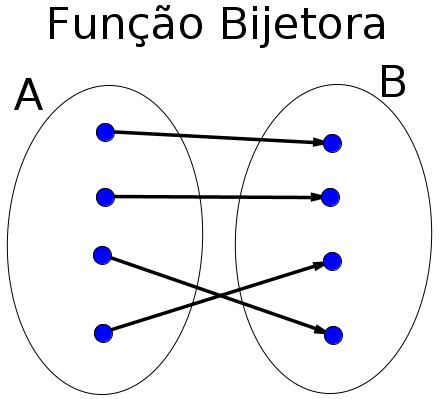
\includegraphics[scale=0.3]{../../imagens/cap21-exercicios-C1-pag160-1.png}
      \caption*{Fonte: Autor}
      \label{cap21-exercicios-C1-pag160-1}
    \end{figure}
    
Vamos descobrir \textbf{quantas funções bijetoras poderemos formar}. Para isso, considere a figura \ref{cap21-exercicios-C1-pag160-2}

   \begin{figure}[!htb]
      \centering
      \caption{[Questão C1, pág.160 2/2 ] - Diagrama de Venn do enunciado da questão}
      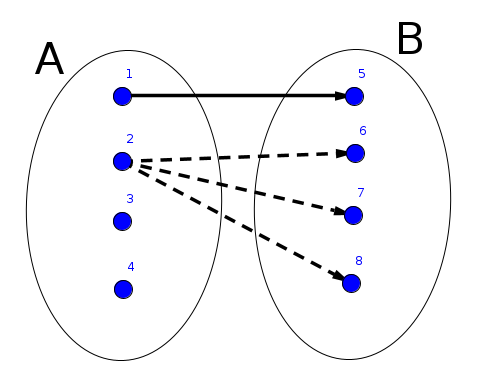
\includegraphics[scale=0.3]{../../imagens/cap21-exercicios-C1-pag160-2.png}
      \caption*{Fonte: Autor}
      \label{cap21-exercicios-C1-pag160-2}
    \end{figure}

\newpage    
    
\begin{center}
{\large \textbf{Resolução da Questão}}
\end{center}    
   
   \begin{itemize}
     \item[\ding{172}] \textbf{O que contar?} Quantas funções bijetoras poderemos formar.
    \item[\ding{173}] \textbf{Restrições do(s) Experimento(s):} A função deve ser bijetora.
        \begin{enumerate}[a)]
          \item Cada elemento do domínio A só pode ser levado a um elemento do contradomínio B (Para ser uma relação do tipo função)
          \item Cada elemento do contradomínio B só pode estar ligado a um elemento do domínio A ( função injetora )
          \item Não pode sobrar elementos no contradomínio B ( função sobrejetora )          
        \end{enumerate}      
     \item[\ding{174}] \textbf{Experimento 1:} $E_1$ = Para o primeiro elemento do domínio "1" em $ A$, devemos escolher um elemento do contradomínio em $B$ de forma a respeitar a restrição do enununciado da questão. Essa escolha gera $n_1 = 4$ possibilidades de escolha no contradomínio.
     \item[\ding{175}] \textbf{Experimento 2:} $E_2$ = Para o segundo elemento do domínio "2" em $ A$, devemos escolher um elemento do contradomínio em $B$ de forma a respeitar a restrição do enununciado da questão. Essa escolha gera $n_2 = 3$ possibilidades de escolha no contradomínio, pois um elemento já foram escolhida no $E_1$.
     \item[\ding{176}] \textbf{Experimento 3:} $E_3$ = Para o terceiro elemento do domínio "3" em $ A$, devemos escolher um elemento do contradomínio em $B$ de forma a respeitar a restrição do enununciado da questão. Essa escolha gera $n_3 = 2$ possibilidades de escolha no contradomínio, pois dois elementos já foram escolhidos no $E_1 \textrm{ e } E_2$.
     \item[\ding{177}] \textbf{Experimento 4:} $E_4$ = Para o quarto elemento do domínio "4" em $ A$, devemos escolher um elemento do contradomínio em $B$ de forma a respeitar a restrição do enununciado da questão. Essa escolha gera $n_4 = 1$ possibilidade de escolha no contradomínio, pois três elementos já foram escolhidos no $E_1 \textrm{ e } E_2 \textrm{ e } E_3$.
         \item[\ding{176}] \textbf{Cálculo:} Pelo princípio fundamental da contagem (PFC), o experimento $E_1$ possui $n_1$ resultados possíveis, o experimento $E_2$ possui $n_2$ resultados possíveis, o experimento $E_3$ possui $n_3$ resultados possíveis e o experimento $E_4$ possui $n_4$ resultados possíveis, logo o experimento composto $E_1, E_2, E_3 \textrm{ e } E_4$, nessa ordem, apresenta $n_1 \times n_2 \times n_3 \times n_4$ resultados possíveis, ou seja, $4 \times 3 \times 2 \times 1 = 24$ resultados possíveis.
    \item[\ding{177}] \textbf{Conclusão:} Podemos formar 24 funções bijetoras com os conjuntos A e B (domínio e contradomínio, respectivamente).

   \end{itemize}  
    

\item[\textbf{C2}] Quantas funções injetoras podem ser definidas em $A = \{1, 2, 3, 4\}$ com imagens em $B = \{a, b, c, d, e, f\}$? 

\item[\textbf{C3}] Quantos subconjuntos tem o conjunto $A = \{a, b, c, d, e\}$? 

\item[\textbf{C4}] O número $n = 2^x \times 3^4 \times 5^2 \textrm{, com } x \in \mathbb{N}$, possui sessenta divisores naturais. Determine $x$. 

\item[\textbf{C5}] Quamos números naturais pares de quatro algarismos podem ser formados com os algarismos 1, 2, 3, 4 e 5? 

\item[\textbf{C6}] Quantos números naturais pares de quatro algarismos distintos podem ser formados com os algarismos 1, 2, 3, 4 e 5?

\item[\textbf{C7}] Quantos números naturais maiores do que 400 de três algarismos podem ser formados com os algarismos 1, 2, 4, 5 e 6?

\item[\textbf{C8}] Quantos números naturais maiores do que 400 e de três algarismos distintos podem ser formados com os algarismos 1, 2, 4, 5 e 6? 

\end{enumerate}

\section{Questões de Vestibulares}

\begin{enumerate}

\item[\textbf{V1}]  (UFRS) Dum ponto A a um ponto B existem cinco caminhos; de B a um terceiro ponto C existem seis caminhos, e de C a um quarto ponto D existem também seis caminhos. Quantos caminhos existem para ir do ponto A ao ponto D, passando por B e C?
  \begin{enumerate}[a)]
    \item 17
    \item 30
    \item 180
    \item 680
    \item 4080
  \end{enumerate}  
 
\item[\textbf{V2}] (FGV-SP) Antes de 1990 as placas de automóveis eram constituídas de duas leuas seguidas de quarto algarismos. Quantas placas desse tipo, diferentes, podem ser formadas com as vogais do afabeto e algarismos pares?
  \begin{enumerate}[a)]
    \item 400
    \item 31250
    \item 7812
    \item 15625
    \item n.d.a. 
  \end{enumerate} 
 
\item[\textbf{V2}] (Vunesp) Os jomais noticiaram que, a partir de 1990, o código de placas dos automóveis particulares seda constituído por três letras seguidas de quatro algarismos, admitindo-se repetições. Usando-se 26 letras e dez algarismos, o maior número possível de placas desse tipo em que figuram pelo menos uma lona R e pelo menos uma letra C é:

  \begin{enumerate}[a)]
    \item $32 \times 35 \times 10^4$
    \item $3 \times 2 \times 26 \times 10^4$
    \item $3 \times 26 \times 10^4$
    \item $325 \times  24 \times 23 \times 10^4 $
    \item $41 \times 6 \times 10^4 $
  \end{enumerate} 

\item[\textbf{V2}]  (PUC-MG) Considerando os elementos do conjunto A = 10, 1, 2, 4, 5, 6, 7, 91, quantos números inteiros de cinco algarismos distintos, maiores que 64000, podem ser formados? 

\item[\textbf{V2}] (Cesgranrio) Considere todos os n números pares positivos, de quatro dígitos distintos, formados com os algarismos I, 2, 3 e 4. Então $n$ é:
  \begin{enumerate}[a)]
    \item 10
    \item 12
    \item 16
    \item 18
    \item 24 
  \end{enumerate} 

\end{enumerate}


%
% --------------------   ESTRUTURA PADRÃO DE UMA QUESTÃO  ------------------------
% Observação: 
%    1) O "\item" abaixo precisa estar dentro de um \begin{itemize} ... \end{itemize}
%    2) Use CTRL + T para COMENTAR e CTRL + U para DESCOMENTAR
%    3) A resolução de uma questão é dividida da seguinte forma:
%      a) Enunciado da Questão
%      b) Apresentação de alguma figura (ilustração, esquema, mapamental) para auxiliar a resolução
%      c) Passos de 1 a 10 para resolver a questão
% Nota: Capture a tela com as questões do livro e use a ferramenta "https://www.onlineocr.net/pt/" para fazer o reconhecimento de caracteres.
%
%\item[\textbf{QXX}] Coloque aqui o enunciado da questão ... ?
%   \begin{itemize}
%    \item[\ding{172}] \textbf{O que contar?:} .
%    
%    \item[\ding{173}] \textbf{Restrições do(s) Experimento(s):} .
%    
%    \item[\ding{174}] \textbf{Experimento 1:} $E_1$ = Preencher a posição das unidades com um dos algarismos dados.\\ Sendo $n_{1}$ o número de resultados possíveis do \textbf{experimento 1}, $n_{1}$ possui $n(A)$ resultados possíveis, ou seja, $n_{1} = n(A) = 5$.
%    
%    \item[\ding{175}] \textbf{Experimento 2:} $E_2$ = Preencher a posição das dezenas com um dos algarismos dados.\\ Sendo $n_{2}$ o número de resultados possíveis do \textbf{experimento 2}, $n_{2}$ possui $n(A)-1$ resultados possíveis,pois um dos algarismos já foi escolhido no experimento 1, ou seja, $n_{2} = n(A)-1 = 5 - 1 = 4$.
%    
%    \item[\ding{176}] \textbf{Experimento 3:} $E_3$ = Preencher a posição das centenas com um dos algarismos dados.\\ Sendo $n_{3}$ o número de resultados possíveis do \textbf{experimento 3}, $n_{3}$ possui $n(A)-2$ resultados possíveis,pois um dos algarismos já foi escolhido no \textbf{experimento 1} e outro no \textbf{experimento 2}, ou seja, $n_{2} = n(A) - 2 = 5 - 2 = 3$.   
%    
%    \item[\ding{177}] \textbf{Cálculo:} Pelo princípio fundamental da contagem (PFC), os experimentos 1, 2 e 3 apresentam, respectivamente, $n_{1},\, n_{2} \textrm{ e } n_{3}$ resultados possíveis, logo o experimento composto 1, 2 e 3 possuem, nessa ordem, $n_{1} \times n_{2} \times n_{3}$ ou $5 \times 4 \times 3 = 60$ resultados possíveis.
%    
%    \item[\ding{178}] \textbf{Conclusão:} Podemos formar \textbf{60 números naturais de três algarismos distintos} com os números dados.
%    
%  \end{itemize}

\end{document}